\documentclass[10pt]{beamer}
\usetheme{CambridgeUS}
\usecolortheme{beaver}
\usepackage[utf8]{inputenc}
\usepackage{amsmath,amssymb}
\usepackage{graphicx}
\usepackage{booktabs}
\usepackage{hyperref}
\usepackage{listings}
\usepackage{xcolor}\graphicspath{{figures/}}

\title{Predicting Insurance Costs: Analysis and Insights}
\author{SDS Mini-Datathon Team}
\institute[NUS]{National University of Singapore}
\date{\today}

\begin{document}

\begin{frame}
\titlepage
\end{frame}

\begin{frame}{Problem Framing \& Objective}
\begin{itemize}
\item \textbf{Challenge}: Predict medical insurance charges using demographic and lifestyle data
\item \textbf{Goal}: Build accurate regression models and identify key cost drivers
\item \textbf{Importance}: Fair pricing, risk assessment, healthcare insights
\item \textbf{Dataset}: 1,338 records with age, sex, BMI, children, smoker, region, charges
\end{itemize}
\end{frame}

\begin{frame}{Exploratory Data Analysis}
\begin{itemize}
\item Data quality: No missing values, clean dataset
\item Key statistics: Charges range \$1,122--\$63,771 (mean \$13,270)
\item Distribution: Right-skewed charges, normal BMI/age
\end{itemize}
\begin{figure}
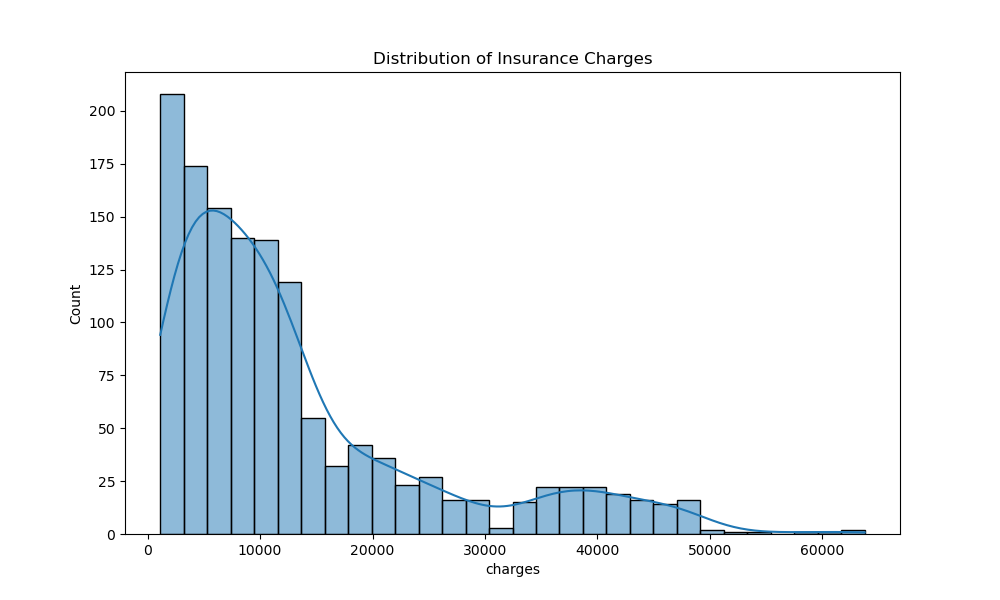
\includegraphics[width=0.8\textwidth]{charges_dist.png}
\caption{Distribution of Insurance Charges}
\end{figure}
\end{frame}

\begin{frame}{Exploratory Data Analysis (Cont.)}
\begin{figure}
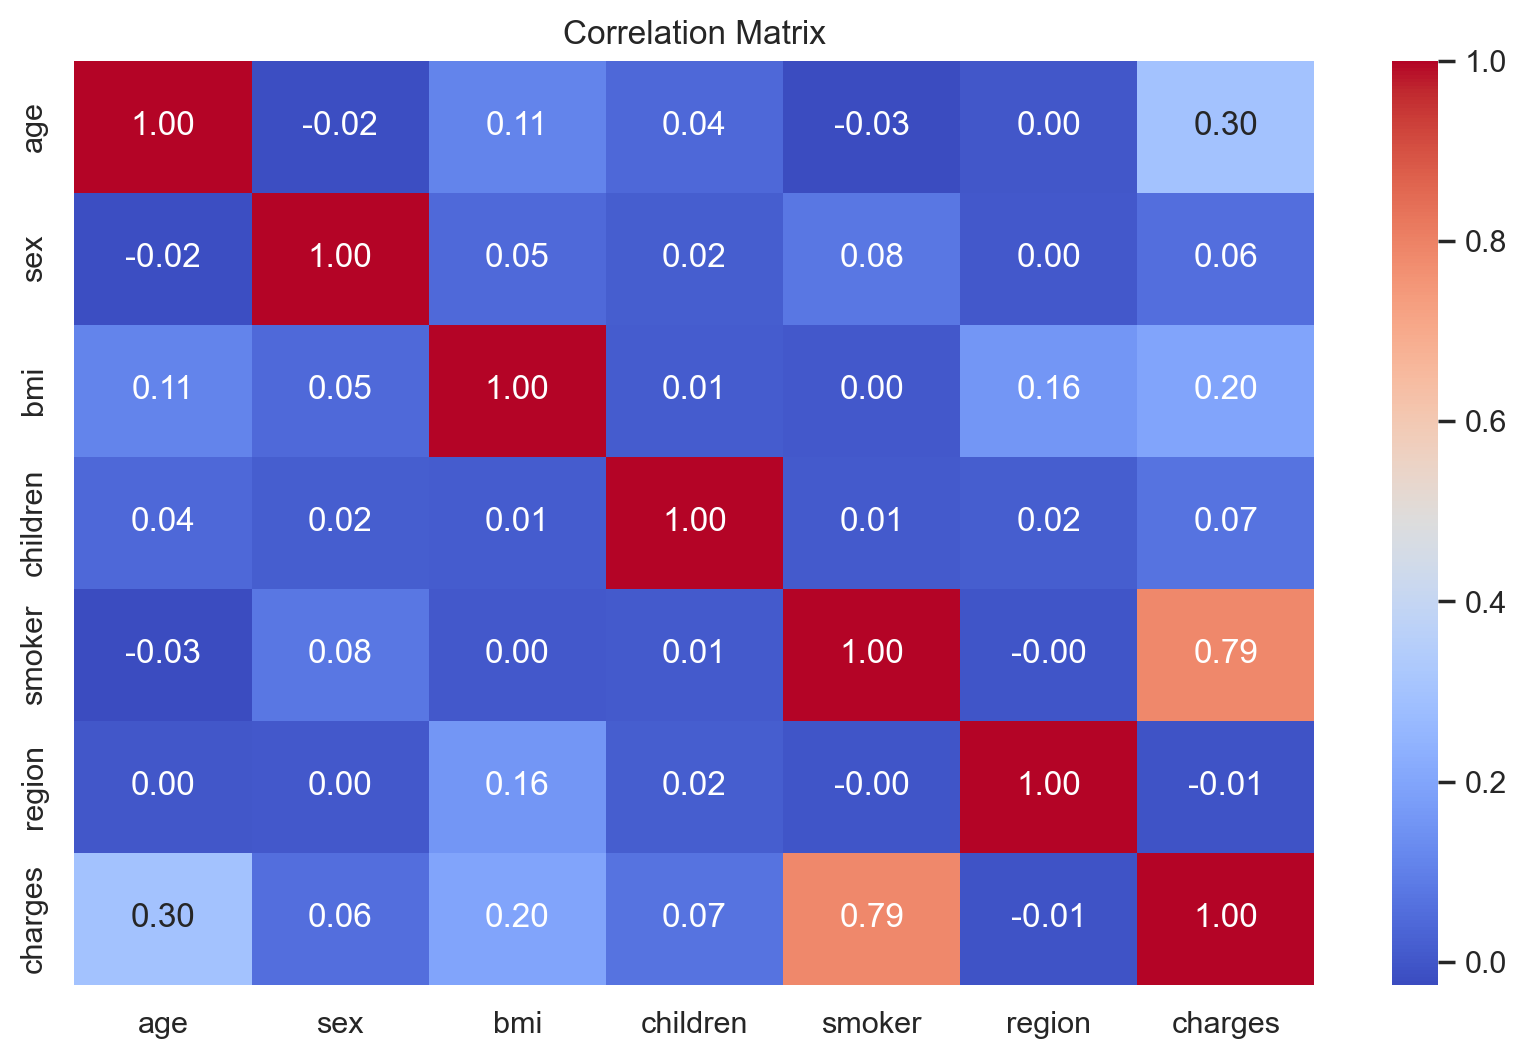
\includegraphics[width=0.8\textwidth]{correlation_heatmap.png}
\caption{Correlation Matrix}
\end{figure}
\begin{itemize}
\item Strong correlations: smoker (+0.79), age (+0.30), BMI (+0.20)
\item Regional variations in charges
\end{itemize}
\end{frame}

\begin{frame}{Regression \& Modeling Approach}
\begin{itemize}
\item \textbf{Baseline Models}:
  \begin{itemize}
  \item Linear Regression: Interpretable, assumes linearity
  \item Decision Tree: Handles non-linearities, prone to overfitting
  \end{itemize}
\item \textbf{Advanced Model}:
  \begin{itemize}
  \item Random Forest: Ensemble of trees, robust and accurate
  \item Hyperparameter tuning with GridSearchCV
  \end{itemize}
\item \textbf{Evaluation}: R², RMSE, MAE; Cross-validation for stability
\end{itemize}
\end{frame}

\begin{frame}{Key Findings \& Visualizations}
\begin{table}[h]
\centering
\begin{tabular}{@{}lccc@{}}
\toprule
Model & R² & RMSE & MAE \\
\midrule
Linear Regression & 0.78 & 5,794 & 4,128 \\
Decision Tree & 0.72 & 6,636 & 3,028 \\
Random Forest & 0.86 & 4,603 & 2,550 \\
\bottomrule
\end{tabular}
\caption{Model Performance Comparison}
\end{table}
\begin{itemize}
\item Random Forest best performer (R²=0.86)
\item Cross-validation confirms stability (CV R²: 0.825 ± 0.085)
\end{itemize}
\end{frame}

\begin{frame}{Feature Impact Analysis}
\begin{figure}
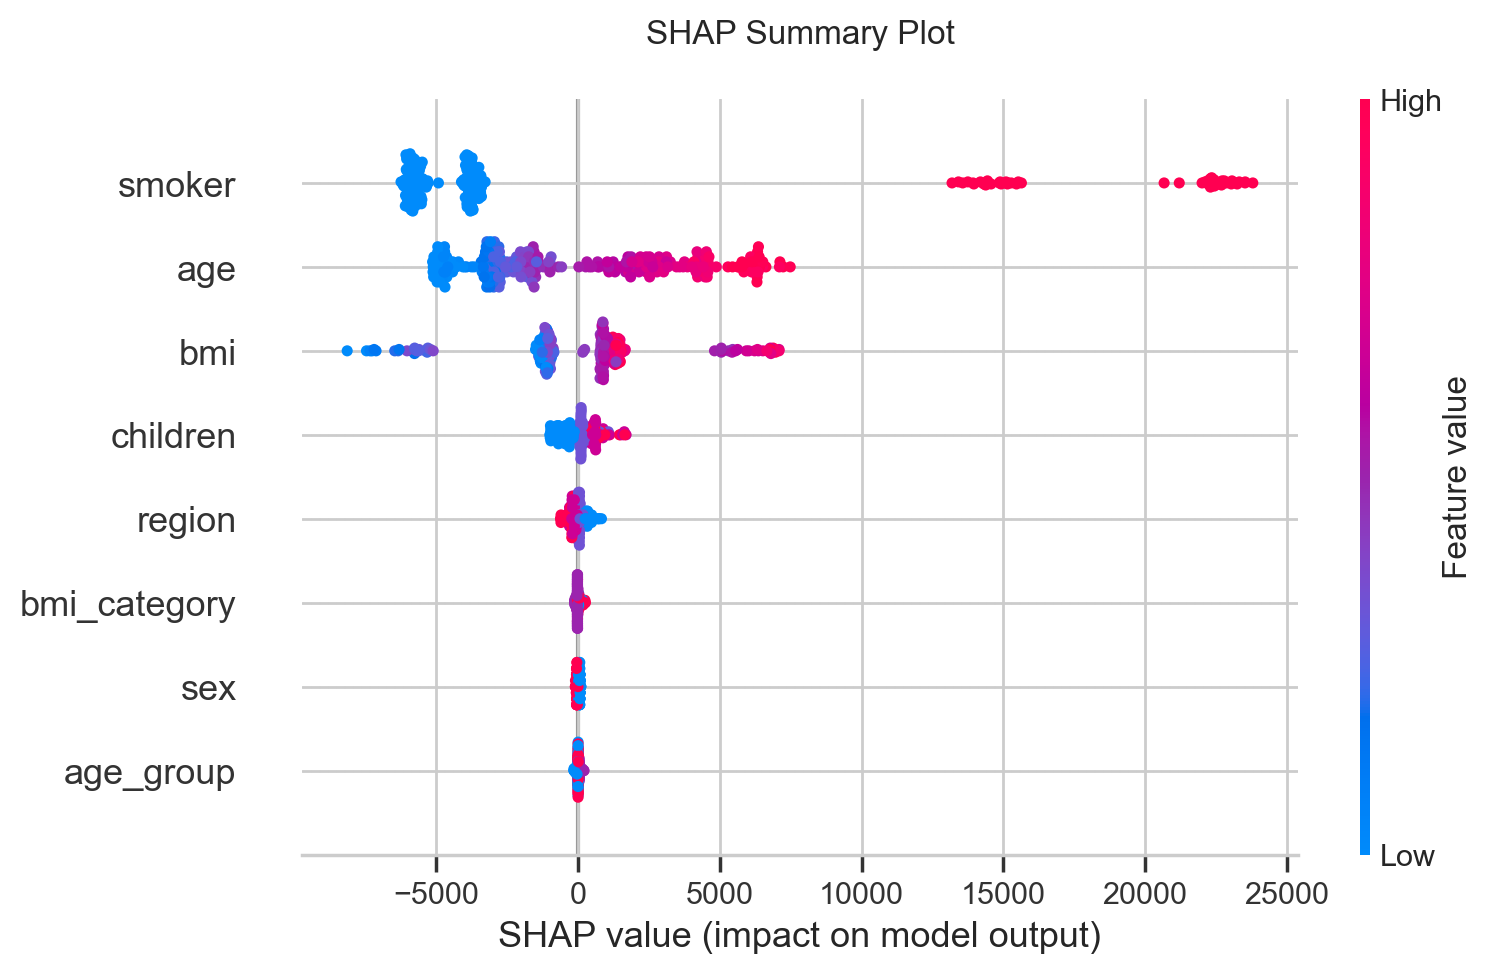
\includegraphics[width=0.8\textwidth]{shap_summary.png}
\caption{SHAP Summary Plot}
\end{figure}
\begin{itemize}
\item Top factors: Smoking (+20k+), Age (+200/year), BMI (+500/unit)
\item SHAP provides individual prediction explanations
\end{itemize}
\end{frame}

\begin{frame}{Fairness Analysis}
\begin{figure}
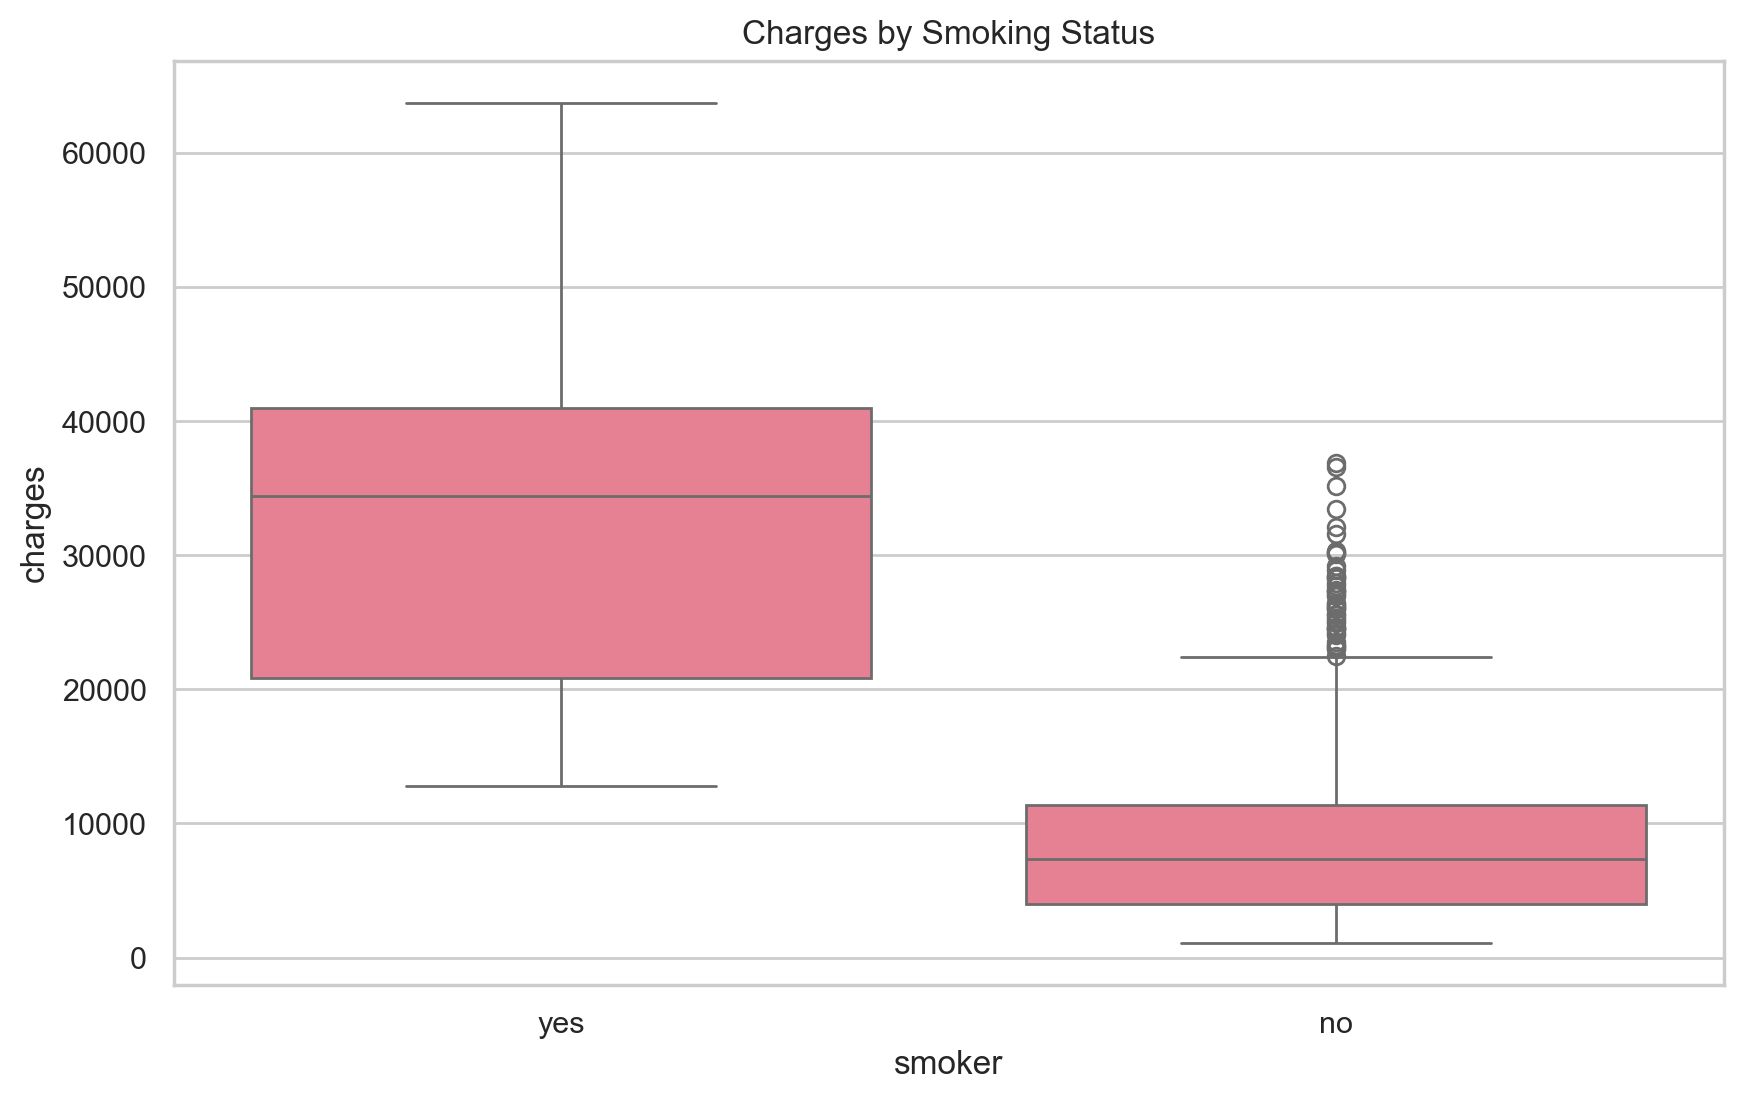
\includegraphics[width=0.8\textwidth]{smoker_boxplot.png}
\caption{Charges by Smoking Status}
\end{figure}
\begin{itemize}
\item Gender gap: Males \$1,387 higher (minimal)
\item Regional differences: Southeast 19\% higher
\item Fairness: Models reflect risk factors, not bias
\item Ethical: Regular audits recommended
\end{itemize}
\end{frame}

\begin{frame}{Practical Recommendations}
\begin{itemize}
\item \textbf{For Insurers}:
  \begin{itemize}
  \item Use Random Forest for premium calculation
  \item Target wellness programs for smokers/high BMI
  \end{itemize}
\item \textbf{Policy Implications}:
  \begin{itemize}
  \item Fair pricing based on verifiable risks
  \item Monitor regional healthcare access disparities
  \end{itemize}
\item \textbf{Future Work}:
  \begin{itemize}
  \item Collect longitudinal data, medical history
  \item Implement advanced models (neural networks)
  \end{itemize}
\end{itemize}
\end{frame}

\begin{frame}{Difficulties Faced \& Solutions}
\begin{itemize}
\item \textbf{Dataset Limitations}:
  \begin{itemize}
  \item Small size (1,338 records) limits generalizability
  \item Missing features: medical history, genetics, lifestyle details
  \item Static data: no temporal health changes
  \end{itemize}
\item \textbf{Technical Challenges}:
  \begin{itemize}
  \item SHAP library version conflicts: Resolved by using compatible API
  \item Model overfitting: Addressed with cross-validation and tuning
  \item Interpretability: Enhanced with SHAP beyond standard methods
  \end{itemize}
\item \textbf{Solutions}:
  \begin{itemize}
  \item Feature engineering for better segmentation
  \item Rigorous validation and error analysis
  \item Innovative explainability techniques
  \end{itemize}
\end{itemize}
\end{frame}

\begin{frame}{Conclusion}
\begin{itemize}
\item Successfully predicted 86\% of insurance cost variance
\item Smoking is the dominant factor, followed by age and BMI
\item Models are fair and practical for real-world use
\item Future: Larger datasets and advanced AI for better accuracy
\end{itemize}
\begin{center}
Thank you for your attention!
\end{center}
\end{frame}

\end{document}